\chapter{Exigences non fonctionnelles}
Dans ce chapitre, les différentes exigences non fonctionnelles qui ont été sélectionnées seront explicitées. Pour rappel, de telles exigences décrivent les propriétés que le produit doit respecter. Pour ce faire, plusieurs de ces qualités ont été sélectionnées dans le modèle de Volere et seront présentées ci-dessous.

\section{Ergonomie et convivialité du produit}
SportEasy étant destiné à être une application sur smartphone, les couleurs, les interfaces et tout ce qui touche au visuel seront les premières choses que percevront les utilisateurs. Il est donc plus qu'important de définir quelque chose de plaisant et d'agréable afin de tout de suite accrocher le potentiel sportif et gagner le pas sur la concurrence. Afin de maximiser l'expérience de l'utilisateur et les chances de survie de l'application, il faut que les interfaces respectent certaines contraintes et que le packaging du produit soit attrayant.

\subsection*{Interface}
Cette application a pour vocation de configurer des séances sportives pour des utilisateurs aguerris ou non, comme il l'a déjà été mentionné plusieurs fois plus haut dans ce travail. Dès lors, il est nécessaire que son emploi soit rapide et intuitif et ne nécessite pas de lectures fastidieuses. Dès lors, il est important que la majorité de l'application soit graphique et compréhensible en un coup d'\oe il.\\

\'Etant donné que l'étude de partenariat n'a été menée que dans le cadre de la Belgique, notamment en Wallonie, il est normal que les interfaces soient définies, dans un premier temps, en français. Cependant, afin de toucher plus de monde, il est nécessaire de traduire ces interfaces le plus vite possible dans des langues plus accessibles (l'anglais, principalement, afin de devenir rapidement international).\\

La Figure \ref{fig:interfaces} montre des prototypes d'interfaces (qui ont d'ailleurs été plus détaillés dans le chapitre précédent). Ces IHM sont en accord avec la vision que le produit doit avoir : simples, sobres et efficaces.

\begin{figure}[!h]
	\centering
	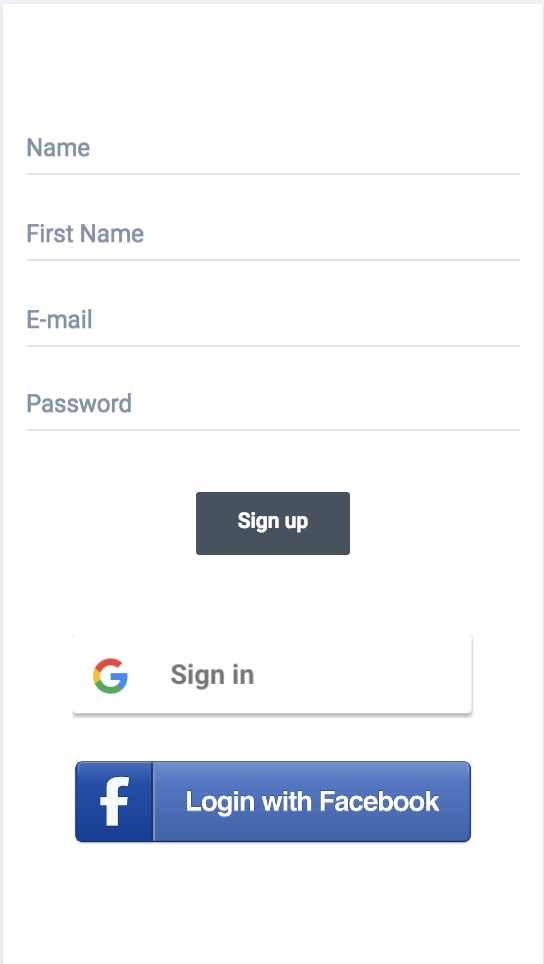
\includegraphics[scale=0.3]{ihms/inscription}
	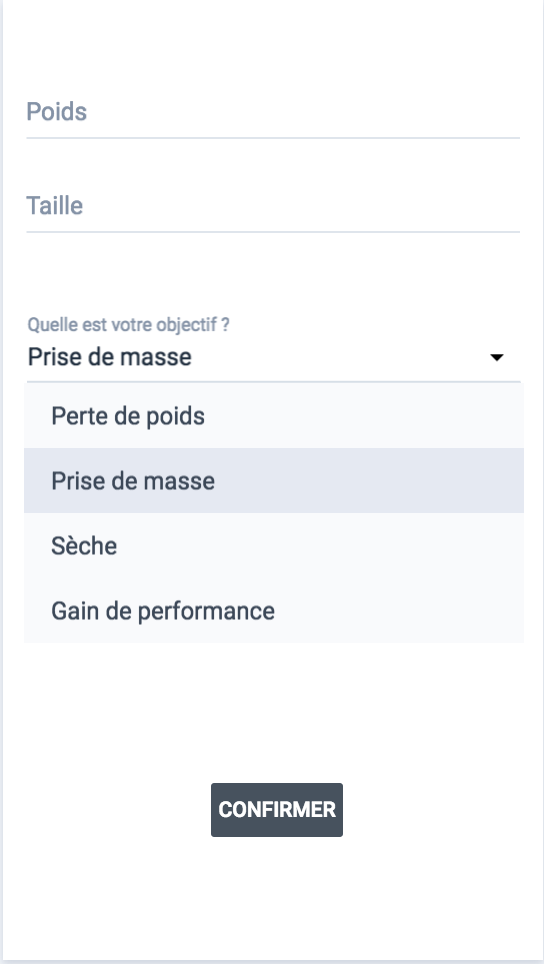
\includegraphics[scale=0.3]{ihms/caracteristiques}
	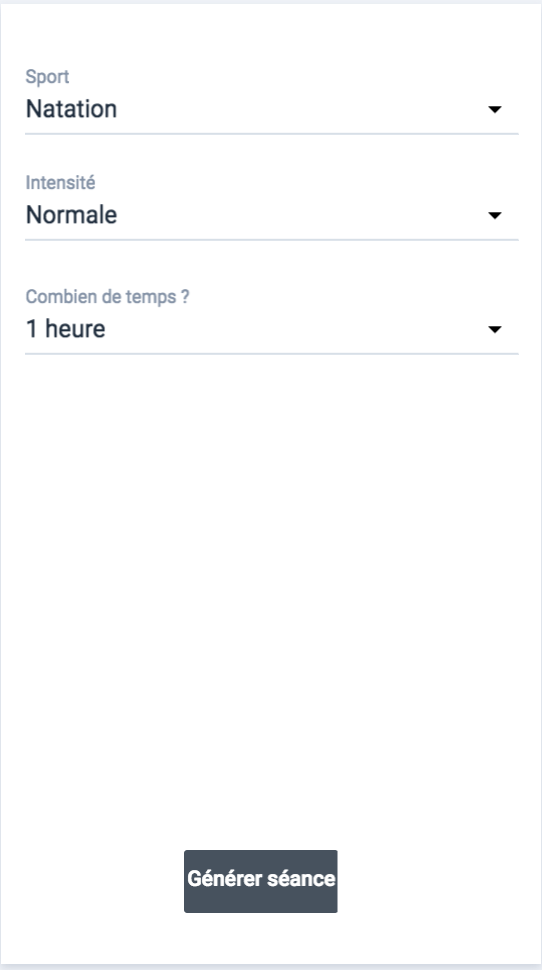
\includegraphics[scale=0.3]{ihms/seance}
	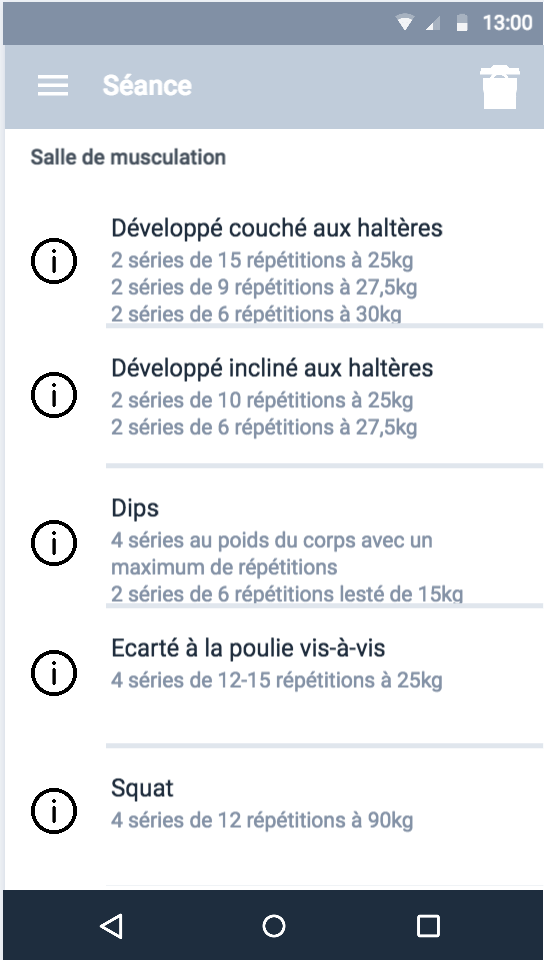
\includegraphics[scale=0.3]{ihms/normal_session}
	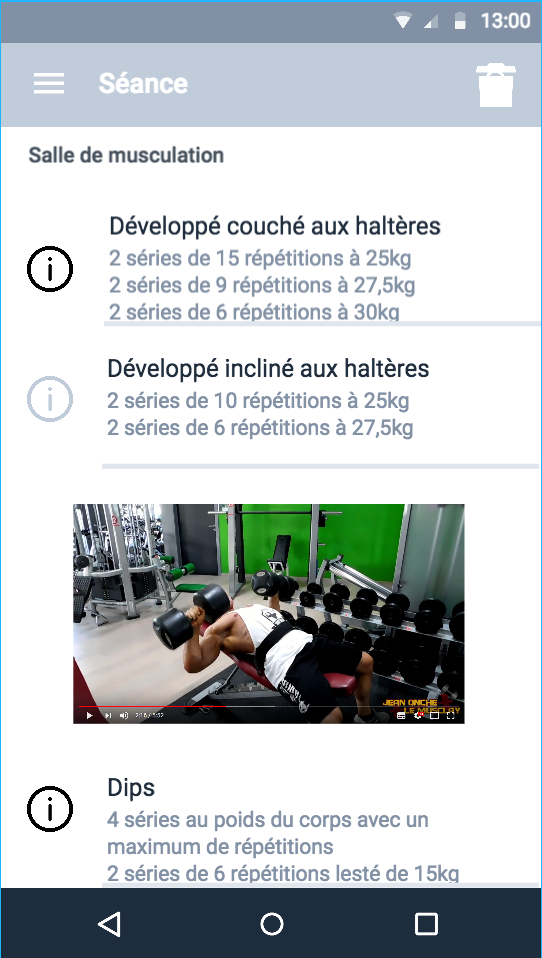
\includegraphics[scale=0.3]{ihms/get_information_about_exo}
	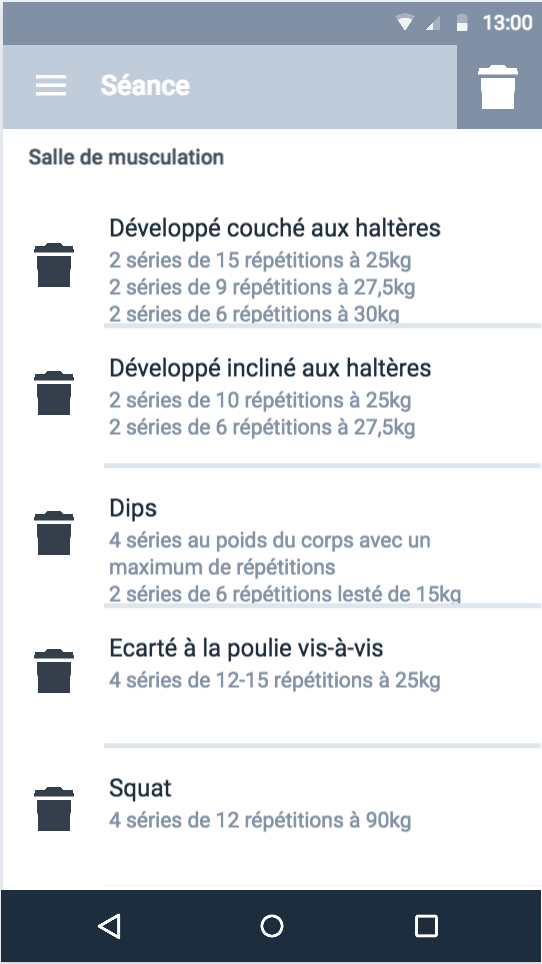
\includegraphics[scale=0.3]{ihms/remove_exo}
	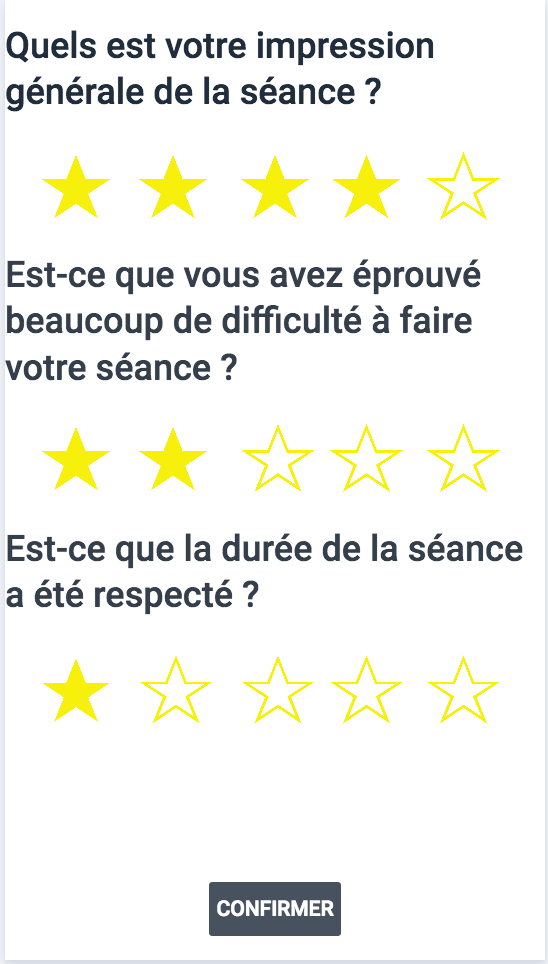
\includegraphics[scale=0.3]{ihms/rating_before_update}
	\caption{\label{fig:interfaces}Interfaces}
\end{figure}

\subsection*{Style et packaging du produit}
S'il est difficilement envisageable de définir un packaging pour une application mobile, il est néanmoins primordial que le produit respecte quelques conditions de style afin d'être un succès une fois lancé sur le marché.\\

Ainsi, le produit doit avoir l'air moderne et dynamique. Il est donc nécessaire que ce dernier respecte les dernières tendances en matière d'applications mobiles afin de se frayer un chemin aisé sur le marché et ne pas être désuet avant même d'avoir existé.\\

De même, bien que l'application soit destinée à toute personne souhaitant faire du sport, elle touchera rarement les enfants, qui nécessitent une attention particulière dans leur séance sportive de part leur croissance toujours bien active. Dès lors, l'application ne doit pas présenter de couleurs particulièrement \og flashy \fg{}.\\

Enfin, il est important que le produit suscite l'envie de faire du sport et stimule la motivation de l'utilisateur. Pour se faire, il doit employer un design frais, dynamique et énergétique tout en étant présenté de façon motivante. Le tout est que l'utilisateur ait envie de se lever pour faire du sport à peine ayant eu accès à l'application.

\section{Facilité d'utilisation et facteurs humains}
- Facilité d'utilisation
- Personnalisation
- Facilité d'apprentissage
- Facilité de compréhension et de politesse
- Exigences d'accessibilité

\section{Performances du produit}
- Rapidité et temps de latence
- Sécurité
- Précision et exactitude
- Fiabilité et disponibilité
- Robustesse et tolérance à un emploi erroné
- Capacité de stockage et montée en charge
- Adaptation du produit à une augmentation de volume à gérer
- Longévité

\section{Adéquation du produit avec son environnement}
- Environnement physique
- Environnement technologique
- Applications "partenaires" (collaboration)
- Commercialisation

\section{Maintenance et support du produit}
- Maintenance
- Conditions spéciales de la maintenance
- Exigences en matière de support
- Exigences de portabilité
- Installation du système

\section{Sécurité}
- Accès au système
- Intégrité
- Protection des données à caractère personnel
- Audit et traçabilité
- Protection contre les infections

\section{Exigences culturelles et politiques}
- Exigences culturelles
- Exigences politiques

\section{Lois et standards}
- Conformité avec la loi
- Conformité avec des standards